\subsection{Methane decomposition using a hydroxyapatite supported nickel catalyst.}%
\label{sub:methane_decomposition_using_a_hydroxyapatite_supported_nickel_catalyst_}

One method of methane decomposition currently relies on a nickel catalyst, supported by compounds such as \ce{TiO2}, \ce{MgO}, \ce{ZrO2}, \ce{Al2O3}. The rate of reaction depends on the \ce{Ni} particle size, with both relation to the dispersion and stabilisation by a suitable support. \cite{Ashok}
 J. Ashok, S Naveen. Kumar, M. Subrahmanyam, A. Venugopal, have been looking at how a new nickel catalyst support, hydroxyapatite (HAp), and how it will affect this reaction. \ce{HAp} is produced from \ce{Ca5(NO3)4O.4H2O} and \ce{(NH4)(PO3OH)} to make \ce{[Ca5(PO4)3(OH)]} while under basic conditions.\cite{Ashok}
Unlike the previously mentioned catalyst supports, \ce{HAp} is irreducible; this means no \ce{CO} is made in the reaction unlike the other supports currently in use, meaning the reaction has a simple overall equation with no greenhouse gas (GHGs) emissions:

\begin{align}
	\ce{CH4 -> C +2H2}
.\end{align}

This reaction has an enthalpy of \SI{75.6}{\kilo\joule\per\mole} meaning it is endothermic. In the experiment performed by J. Ashok et al. the experiment was run at just \SI{650}{\celsius} \cite{Ashok}, as this is an endothermic reaction these operating condition are fairly mild. The \ce{CH4} should be flowed through the reaction chamber at a fairly slow \SI{24}{\liter\per\hour} \cite{Ashok} again meaning no extra energy is needed to accelerate the gas. These combined factors and the lack of (GHGs) produced make this reaction both green and sustainable.

\begin{figure}[H]
	\centering
	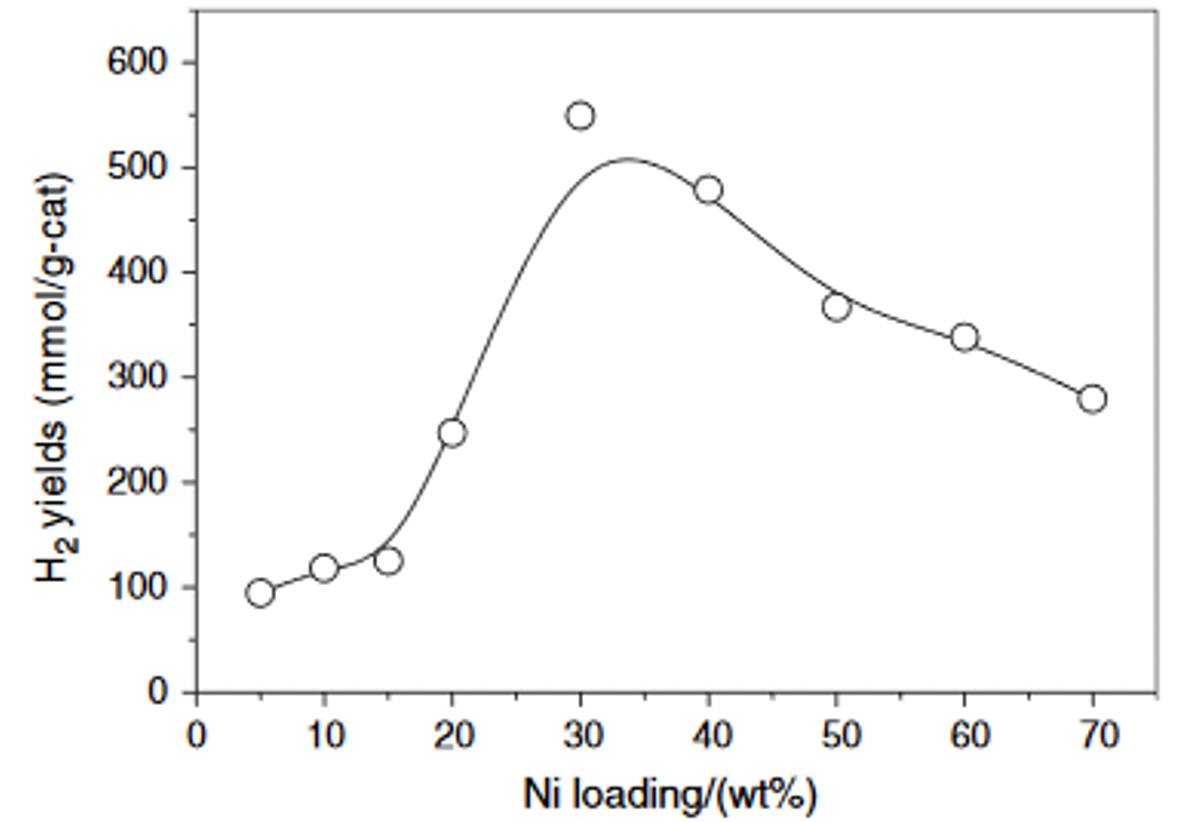
\includegraphics[width=0.4\textwidth]{539a7840-2cb8-11eb-895f-8c8590753a48.png}
	\caption{A plot of percent weight of nickel loaded onto the catalyst support vs \ce{H2} yield.}  
	\label{fig:MD_plot1}
\end{figure}

\begin{figure}[H]
	\centering
	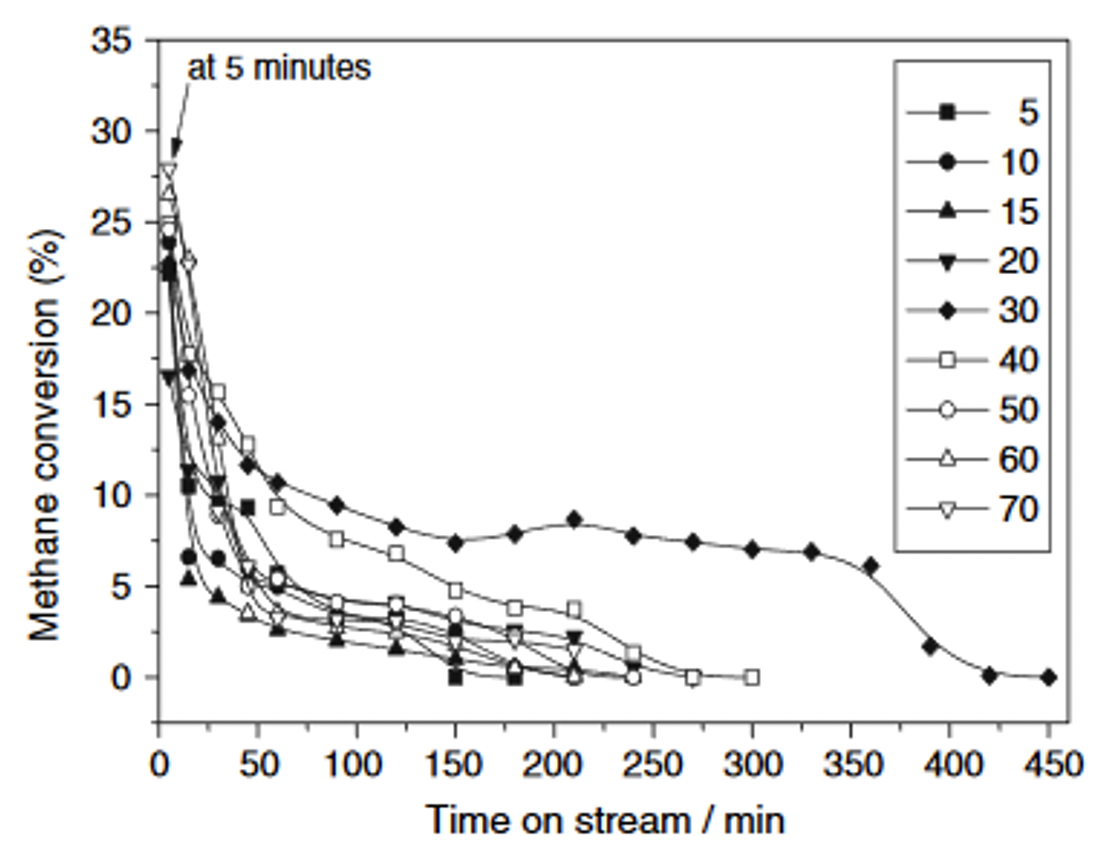
\includegraphics[width=0.4\textwidth]{0ed19cac-2cb8-11eb-895f-8c8590753a48.png}
	\caption{A multiple plot of varying percent weights of nickel loaded onto the support showing how methane conversion efficiency varies with time.}
	\label{fig:MD_plot2}
\end{figure}

As you can see from figures \ref{fig:MD_plot1} and \ref{fig:MD_plot2} a 30 wt\% \ce{Ni} sample was the optimum for this reaction. It has both the highest yield and the best durability. This reaction does have one major draw back however in that the catalyst does readily degrade. This means the solid waste carbon, which is responsible for the deactivation of the catalyst, will be contaminated with toxic \ce{Ni} atoms.
This is a very promising technology which warrants further research, as it can help to solve the current \ce{H2} crisis.


\subsection{Radical chain reactions}%
\label{sub:radical_chain_reactions}

Radical methane pyrolysis is a way of breaking a \ce{CH4} molecule into \ce{H2} and pure carbon.
The initial step is the chemisorption of \ce{CH4}, onto the surface of the catalyst.

\begin{align}
	\intertext{The initiation and rate determining step of the radical break down is:}
	\ce{CH4&-> ^.CH3 + H^.}
	\intertext{Then a series of propagation steps take place with the general equation:}
	\ce{^.CH_{n}&-> ^.CH_{n-1} + H^.}
	\intertext{Until a termination step is reached:}
	\ce{4H^.&-> 2H2}
	\intertext{This gives the overall equation of:}
	\ce{CH4&-> C + 2H2}
.\end{align}

This reaction mechanism gives rise to no waste gases such as \ce{CO2} but does has the issue of elemental carbon production which can lead to the degradation of the catalyst as carbon is deposited upon the catalyst surface.
The reaction conditions for this mechanism follow Le Chatelier’s principal.
As the reaction is endothermic a high temperature is needed, as there are more moles on the RHS, low pressure is needed.
This is very expensive to maintain.
The methane should also move at a low velocity as increases the contact efficiency between the methane and the catalyst, this results in a higher quantity of methane being adsorbed on the active site of the catalyst which means the catalyst will deteriorate slower.

Various catalysts can be used from metals, molten salts/ metals, or carbon-based catalysts.
The main catalysts in a metal catalysed reaction are nickel and iron, these are particularly useful as a partially filled \ce{3d} orbitals accept electrons from the \ce{CH} bonds destabilising their bond strength.
These metals allow carbon diffusion through the crystalline structure.
Table \ref{tab:catalystTable} shows a few key aspects of the catalysts and how they affect the operating conditions and overall reaction process.
\end{multicols}
\begin{table}[H]
	\centering
	\caption{Catalytic efficacies, all relative values are compared to nickel.}
	\label{tab:catalystTable}
	%\resizebox{\columnwidth}{!}
\end{table}
\begin{multicols}{2}

Both supported and non-supported iron catalysts have been tested such as: \ce{[Fe(CO)5]},  \ce{[Fe(cp)2]}.
However, these types of clusters can give result in unwanted gases, meaning the \ce{H2} must be separated from the gaseous mixture.
A catalyst with a strong support increases the carbon dispersion and reducibility of the metal along with preventing sintering of metal particles.
However, an excessively strong support may hamper the reducibility of metal oxides.
A supported catalyst has a better performance as it balances the carbon dispersion resulting in a longer lasting catalyst while maintaining the reducibility of the metal species.

There are three types of carbon catalyst highly ordered, less ordered, and disordered.
Disordered carbon catalysts have three valence sites or no coordination sites these are known as high energy sites (HES).
The more HES’s there are the faster the rate as these are thought to initiate the mechanism.
More oxygenated catalysts have a higher activity but release \ce{COx}, this is because as \ce{COx} is produced new active sites are created on the surface of the catalyst.

\subsection{Discussion of methane methods}%
\label{sub:discussion_of_methane_methods}

CH4 provides a very good solution to the hydrogen problem.
The feedstock while less common and renewable than water, can provide a reliable \ce{H2} supply to locations with poor access to water or an unreliable electricity supply.

\begin{figure}[H]
	\centering
	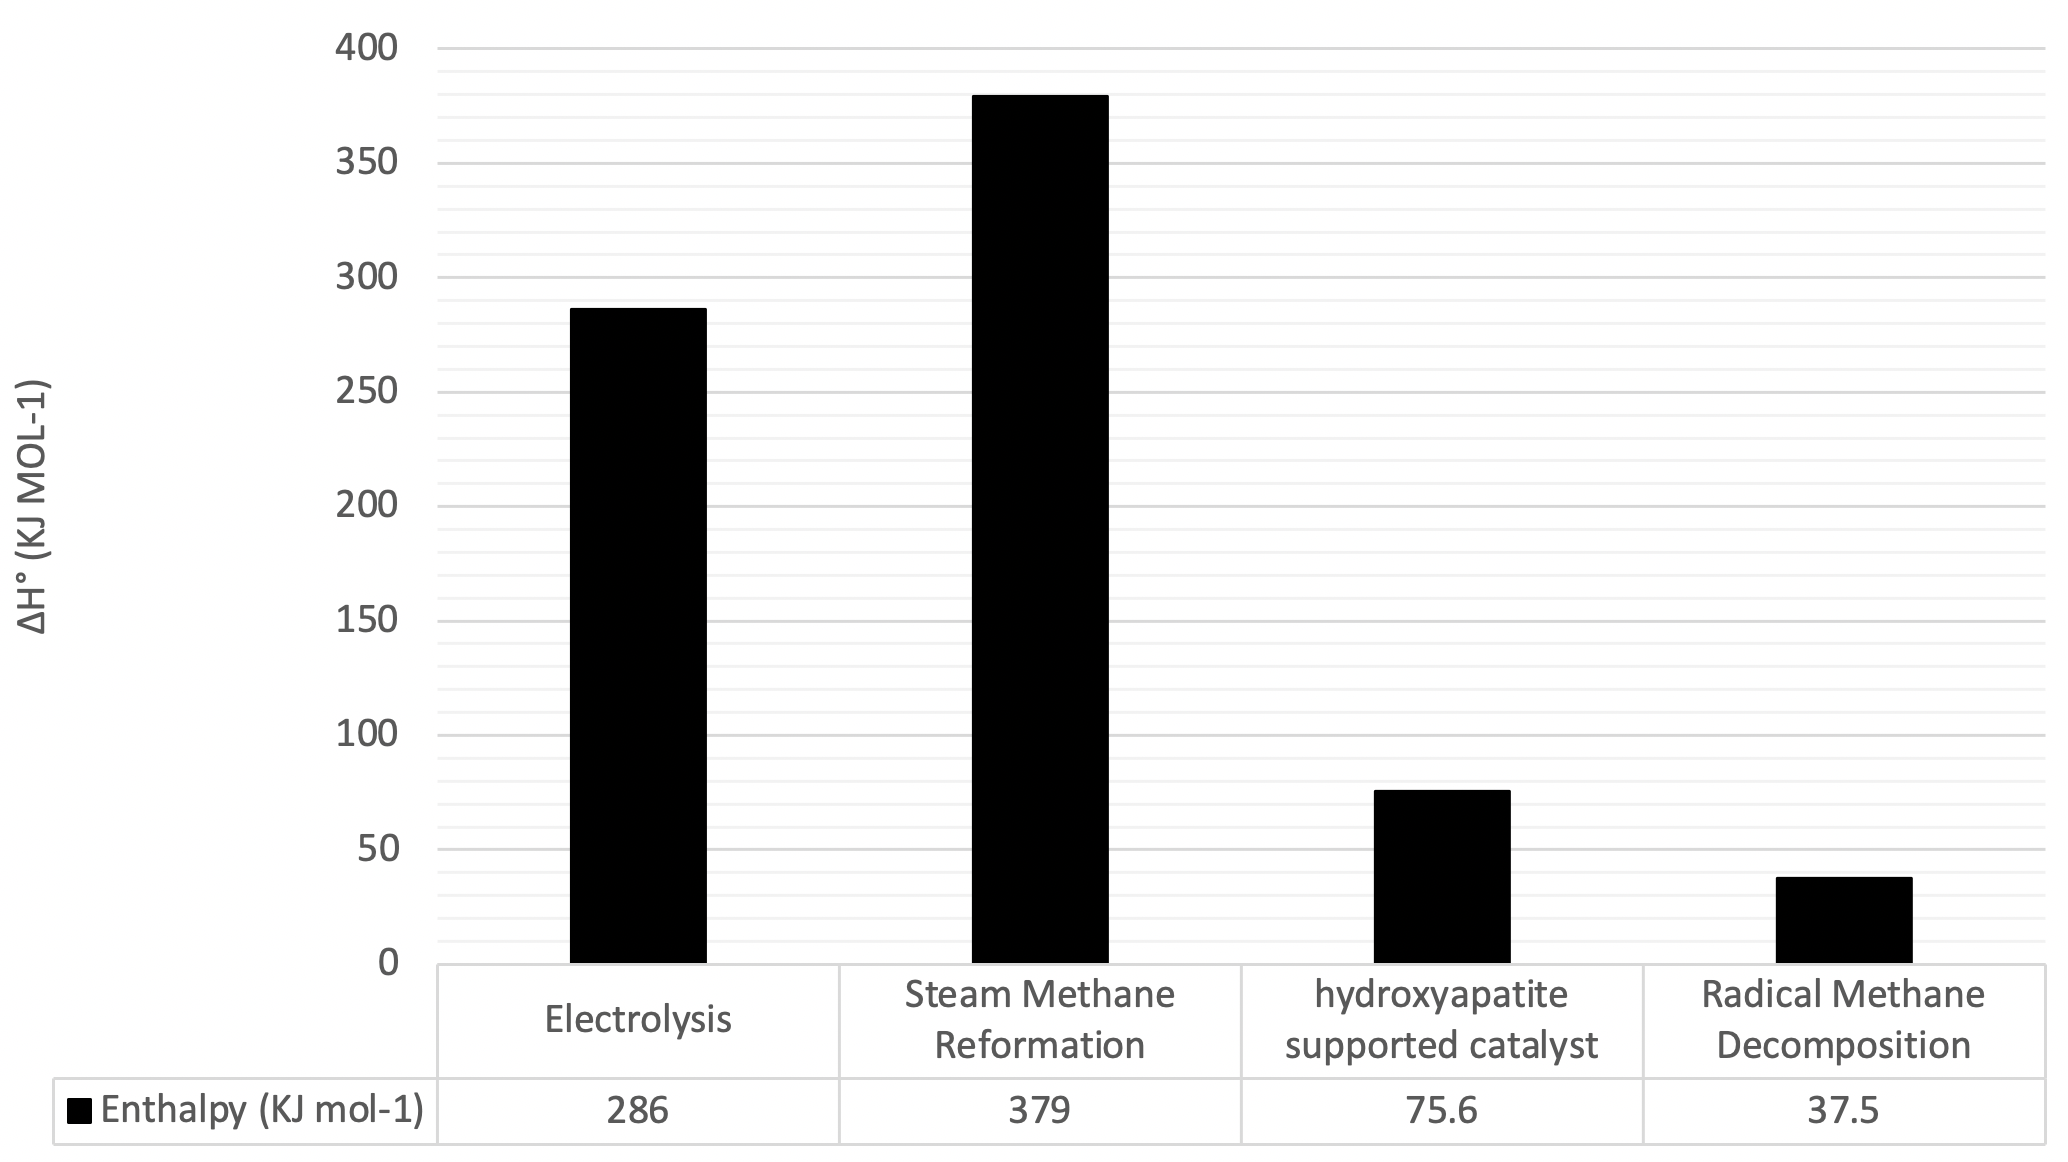
\includegraphics[width=0.4\textwidth]{6b76c760-2cb9-11eb-895f-8c8590753a48.png}
	\caption{A plot showing the enthalpy of the three methane methods alongside uncatalyzed electrolysis as a reference.\cite{SBN2020,Ashok,Saxena2011}}
	\label{fig:ME_disc}
\end{figure}

As you can see from \ref{fig:ME_disc}, radical methane decomposition and hydroxyapatite supported \ce{Ni} catalysts have a significantly lower enthalpy cost meaning they are far more economical processes.
Both \ce{HAp} and RMD both run at much lower operating conditions compared to SMR, this is beneficial not only to the cost of the reaction, but also to the greenness and sustainability.
Further aiding their sustainability is the lack of greenhouse gases produced by both new reactions.
As there are no GHGs produced in either method, no separation step is required to extract the \ce{H2} gas, another positive when compared to SMR.
There are however drawbacks to the new methods of production.
The produced is not re-sellable for three reasons: there is not a market for it, the carbon rapidly degrades the catalysts and where \ce{Ni} catalysts have been used, the carbon is contaminated with toxic metal.

Therefore, I believe RMD to be a better method than \ce{HAp}.
RMD has the option of using carbon or molten catalysts whereas \ce{HAp} only uses toxic \ce{Ni} catalysts.
The carbon catalysts have a longer life than metals and also run at lower temperatures.
